% =============================================================
%  Case study — the Pugalur--Thrissur link (±320 kV, 2 x 1000 MW,
%  half-bridge MMC symmetrical monopoles, 150 km OHL + 28 km cable).
%  Applies the principles of the preceding subsections to one
%  installation: system parameters, specified recovery times, the
%  recorded durations, the commissioning and field oscillograms, the
%  measured cable stresses and the design decisions of the offer stage.
%  Sources: [24] supplier (Siemens Energy), [25] operator (POWERGRID).
%  Figures: fig/dcf timeline as inline TikZ; fig/w2022_* and fig/k2026_*
%  are the oscillograms of [24] and [25], extracted unchanged.
% =============================================================
\subsection{Case: the Pugalur--Thrissur Link}
\label{sec:dcf-pugalur}

\subsubsection{Reference project}
\label{sec:dcf-pugalur-project}

The Pugalur--Thrissur link connects Pugalur (Tamil Nadu) and North Thrissur
(Kerala) with two independent symmetrical monopoles of 1000\,MW each, at
$\pm$320\,kV, bidirectional, with half-bridge MMC converters and a reactive
power capability of $\pm$1100\,Mvar~[25]. The DC circuit is a hybrid of
150\,km overhead line and 28\,km XLPE cable; a transition station 28\,km
from Thrissur joins the two~[25] (the project map in~[24] gives 143\,km and
32\,km). At Pugalur the link shares the 400\,kV AC bus with the
$\pm$800\,kV, 6000\,MW LCC link from Raigarh. It was commissioned in 2021.
Table~\ref{tab:dcf-system} lists the system parameters the recovery
performance was specified against. The link is thus the configuration of
Sections~\ref{sec:dcf-faults} to~\ref{sec:dcf-alternatives} in every
respect: half-bridge MMC, symmetrical monopole, hybrid DC circuit, and a
parallel link for the power compensation of
Section~\ref{sec:dcf-sequence-compensation}.

\begin{table}[!ht]
  \centering
  \begin{tabular}{@{}l l r r@{}}
    \toprule
    \textbf{Parameter} & & \multicolumn{1}{c}{\textbf{Pugalur}}
      & \multicolumn{1}{c}{\textbf{Thrissur}} \\
    \midrule
    AC voltage, max./min.          & kV   & 440 / 360 & 440 / 360 \\
    AC frequency, max./min.        & Hz   & 52.5 / 47.5 & 52.5 / 47.5 \\
    Negative-sequence voltage      & \%   & 1.5 & 1.5 \\
    Short-circuit power, max./min. & MVA  & 36\,400 / 390 & 36\,400 / 390 \\
    DC voltage, pole to pole       & kV   & \multicolumn{2}{c}{640} \\
    DC current                     & A    & \multicolumn{2}{c}{1563} \\
    Sub-module type                &      & \multicolumn{2}{c}{half-bridge} \\
    \bottomrule
  \end{tabular}
  \caption{System parameters of the Pugalur--Thrissur VSC HVDC link~[25]}
  \label{tab:dcf-system}
\end{table}

\subsubsection{Specified recovery performance}
\label{sec:dcf-pugalur-spec}

The technical specification fixes the times of the three restart attempts
of Section~\ref{sec:dcf-sequence-attempts}, the intervals of the
classification of Section~\ref{sec:dcf-sequence-classification} and the
power compensation of Section~\ref{sec:dcf-sequence-compensation},
Table~\ref{tab:dcf-spec}~[24], [25]. The first restart is to be complete
within 1.5\,s of a pole-to-ground fault and 1.8\,s of a pole-to-pole fault,
including fault clearing and cable discharge. A fault within 15\,min of the
previous one is consecutive; three complete sequences have to be possible
within 45\,min. The active power of the faulted link is to be transferred to
the healthy one within 80\,ms.

\begin{table}[!ht]
  \centering
  \begin{tabularx}{\linewidth}{@{}>{\raggedright\arraybackslash}X l@{}}
    \toprule
    \textbf{Step} & \multicolumn{1}{c}{\textbf{Specified time}} \\
    \midrule
    First restart, pole-to-ground fault (incl.\ fault clearing and
      cable discharge) & $< 1.5$\,s \\
    First restart, pole-to-pole fault & $< 1.8$\,s \\
    Second restart at reduced direct voltage & $> 10$\,s (tap-changer, drive recharge) \\
    Changeover to STATCOM operation & $> 10$\,s \\
    Power compensation by the parallel link & $< 80$\,ms \\
    Consecutive fault & within 15\,min of the previous one \\
    Recovery sequences to be withstood & 3 within 45\,min \\
    \bottomrule
  \end{tabularx}
  \caption{Recovery performance specified for the Pugalur--Thrissur
           link~[24], [25]}
  \label{tab:dcf-spec}
\end{table}

The reduced direct voltage of the second restart is preselected by the
operator between $\pm$256\,kV and $\pm$305\,kV~[24]. The residual-current
identifier of Section~\ref{sec:dcf-zones-identification} covers fault
impedances up to 5\,k$\Omega$ on this link~[24]. The discharge of the
healthy pole is led by the Thrissur station, the Pugalur unit being the
backup~[25]. With no fault impedance, the freewheeling current of a
pole-to-pole fault needs up to 500\,ms to decay~[24].

\subsubsection{Recorded durations of the first restart}
\label{sec:dcf-pugalur-timing}

Figure~\ref{fig:dcf-timing} gives the durations of the four phases of the
first restart after a pole-to-ground fault on the overhead line, as the
operator reports them from the fault records~[25]: fault detection and
converter blocking with the opening of the AC circuit breakers and the
current decay, the discharge and deionisation, the re-energisation through
the insertion resistor up to deblocking, and the power ramp.

\begin{figure}[!ht]
  \centering
  \begin{tikzpicture}[font=\footnotesize, >=Latex,
      ph/.style={draw=atBorderStrong, line width=0.6pt, minimum height=3.9cm,
                 text width=2.55cm, align=left, inner sep=4pt, anchor=north west}]
    \node[ph, fill=atBgSubtle, minimum width=2.9cm] (a) at (0,0)
      {\textbf{Fault detection and converter block}\\[2pt]
       fault detection\\ converter block\\ AC circuit breaker opens\\
       fault current decays ($L/R$)};
    \node[ph, fill=atBgSubtle, minimum width=2.9cm] (b) at (3.0,0)
      {\textbf{Deionisation}\\[2pt]
       discharge unit closes\\ healthy pole discharges\\ fault arc deionises\\
       bypass switch opens};
    \node[ph, fill=atBgSubtle, minimum width=2.9cm] (c) at (6.0,0)
      {\textbf{Recovery}\\[2pt]
       AC circuit breaker closes\\ passive charging through the insertion resistor\\
       bypass switch closes\\ deblock, voltage build-up};
    \node[ph, fill=atBgSubtle, minimum width=2.9cm] (d) at (9.0,0)
      {\textbf{Power transfer}\\[2pt]
       power ramp\\ rebalancing with the parallel link};
    \foreach \n/\t in {a/200--250\,ms, b/250--400\,ms, c/550--580\,ms, d/175\,ms} {
      \draw[<->, atAccentFg, line width=0.7pt]
        ([yshift=0.25cm]\n.north west) -- ([yshift=0.25cm]\n.north east)
        node[midway, above, text=atFg] {\t};
    }
    \draw[->, line width=0.7pt] (0,-4.2) -- (12.0,-4.2) node[right] {$t$};
    \draw (0,-4.3) -- (0,-4.1) node[below=0.2cm] {$t_0$};
  \end{tikzpicture}
  \caption{Phases and durations of the first restart after a pole-to-ground
           fault on the DC overhead line, from the fault records of the
           Pugalur--Thrissur link~[25]}
  \label{fig:dcf-timing}
\end{figure}

\subsubsection{Pole-to-ground fault records}
\label{sec:dcf-pugalur-pg}

The commissioning record in~[24], Figure~\ref{fig:dcf-pg-record}, shows a
first restart with both links at about 50\,\% active and reactive load and
the fault on the positive pole: the pole voltages $U_{dHP}$, $U_{dHN}$, the
pole currents $I_{dHP}$, $I_{dHN}$, the active power of the two links and
their sum, and the reactive power of the two links at each station. The
converters of the faulted link block at the fault instant $t_0$ and the
healthy link takes over the power within the specified time; the active
power of link~2 (red) steps up to carry the total while link~1 (blue)
recovers. The negative pole holds about $-580$\,kV until it is discharged at
$t_0 + 180$\,ms. The circuit breaker of station~A closes and passive
charging starts at $t_0 + 520$\,ms, the bypass switch closes at
$t_0 + 700$\,ms with the deblocking of station~A, and station~B deblocks at
$t_0 + 915$\,ms and restores its reactive power. The active power sharing
between the two links is then restored with the long time constant of
Section~\ref{sec:dcf-sequence-compensation}.

\begin{figure}[!ht]
  \centering
  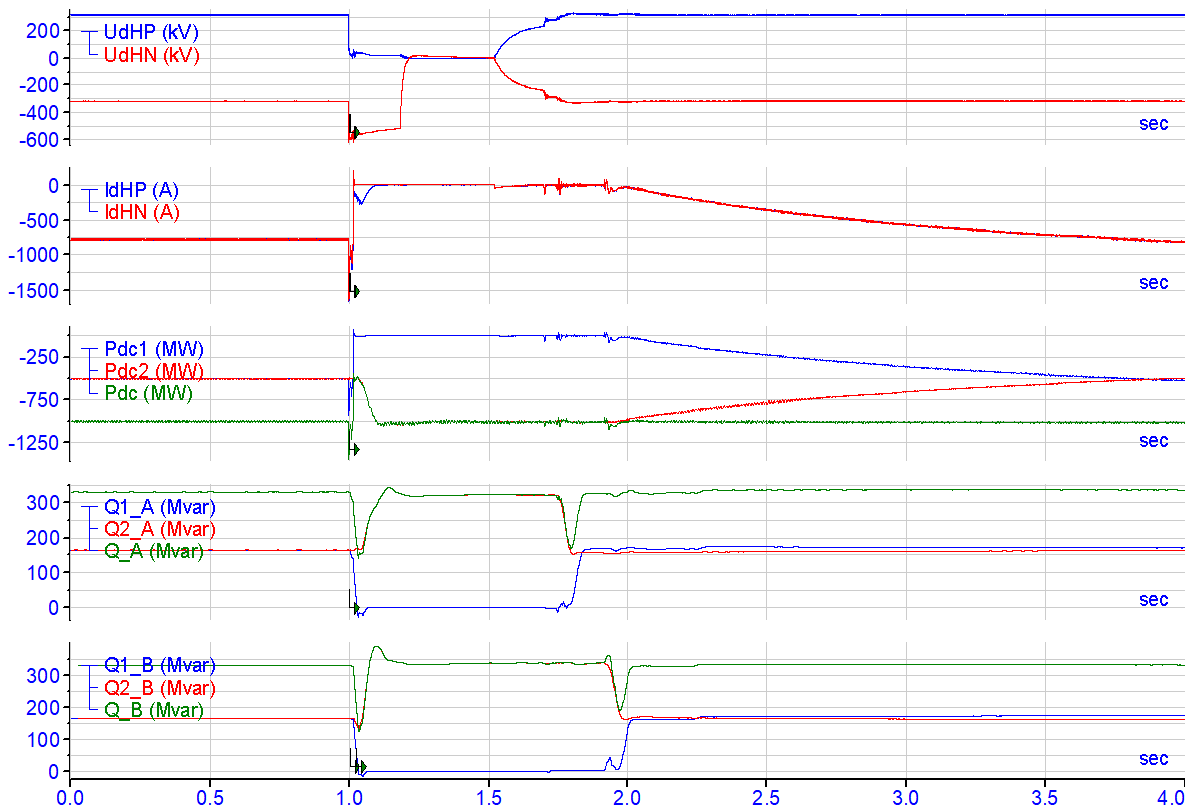
\includegraphics[width=\linewidth]{dc-fault-ride-through/fig/w2022_fig2_pg_recovery.png}
  \caption{Commissioning record of the first restart after a single
           pole-to-ground fault on the positive pole, both links at about
           50\,\% load; from top: pole voltages, pole currents, active power
           of link~1, link~2 and total, reactive power of both links at
           station~A and at station~B. Reproduced from~[24], Figure~2}
  \label{fig:dcf-pg-record}
\end{figure}

Table~\ref{tab:dcf-events} lists the three pole-to-ground faults the
operator evaluated from the transient fault recorder at Pugalur after five
years of service, together with the dynamic performance study case the
control design was validated against~[25]. The three field events share the
same sequence: the healthy pole rises to 600\,kV and is discharged until
$t_0 + 250$\,ms, the deionisation takes about 280\,ms, zone identification
and the reconfiguration request fall into these two intervals, the circuit
breaker recloses with the insertion resistor in circuit for about 200\,ms,
and the converter deblocks between $t_0 + 860$\,ms and $t_0 + 930$\,ms.
Power is restored to the pre-fault level within 2\,s in each case, and the
parallel link carries the power in the meantime. The simulated case at rated
power deblocks within 800\,ms. All recorded first restarts succeeded, and all
lie within the specified 1.5\,s~[25].

\begin{table}[!ht]
  \centering
  \begin{tabular}{@{}l r r r l r r@{}}
    \toprule
    \textbf{Case} & \multicolumn{1}{c}{$P$} & \multicolumn{1}{c}{$Q$}
      & \multicolumn{1}{c}{\textbf{Current}} & \multicolumn{1}{c}{\textbf{Faulted pole}}
      & \multicolumn{1}{c}{\textbf{Deblock}} & \multicolumn{1}{c}{\textbf{Power}} \\
      & \multicolumn{1}{c}{MW} & \multicolumn{1}{c}{Mvar} & \multicolumn{1}{c}{A}
      & & \multicolumn{1}{c}{ms} & \multicolumn{1}{c}{s} \\
    \midrule
    Link~1, field       &  400 & $-150$ &  625 & negative & 930 & 2 \\
    Link~2, field       &  250 &    0   &  390 & positive & 890 & 2 \\
    Link~2, field       &  400 &    0   &  625 & negative & 860 & 2 \\
    Simulation, rated   & 1000 & $+330$ & 1563 & positive & $< 800$ & $\approx 2$ \\
    \bottomrule
  \end{tabular}
  \caption{Recorded and simulated first restarts after a pole-to-ground
           fault on the Pugalur--Thrissur link, reverse power flow Thrissur to
           Pugalur; deblocking time after $t_0$ and time to pre-fault
           power~[25]}
  \label{tab:dcf-events}
\end{table}

Figure~\ref{fig:dcf-pg-tfr} is the transient fault record of the first
event, at 400\,MW on link~1. The positive pole is the healthy one here and
rises to 600\,kV at the fault; the cursors mark 0.722\,s from the fault to
the reclosing of the circuit breaker, 0.193\,s of charging through the
insertion resistor, and 0.932\,s to deblocking. The binary channels below
the analogue traces show the blocking, the zone identification
(\emph{ZONE = DC OHL}), the reconfiguration request and the restart release,
and the positions of the circuit breaker, the bypass switch and the
discharge switch. Figure~\ref{fig:dcf-simulation} is the dynamic
performance study case at rated power the controls were validated against,
with the same sequence and a deblocking within 800\,ms.

\begin{figure}[!ht]
  \centering
  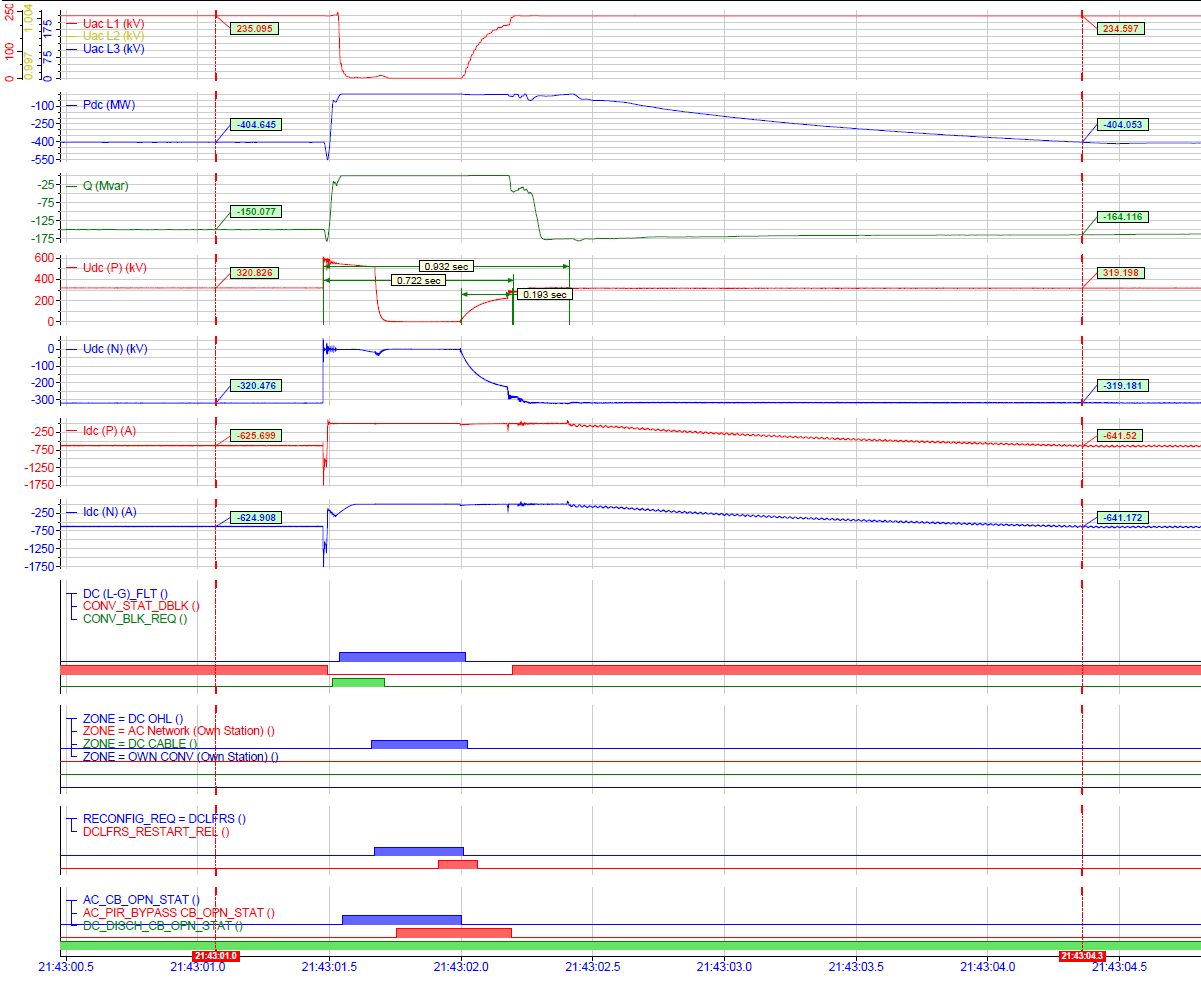
\includegraphics[width=\linewidth]{dc-fault-ride-through/fig/k2026_fig7_tfr_link1_400mw.png}
  \caption{Transient fault record at Pugalur of the pole-to-ground fault on
           the negative pole of link~1 at 400\,MW; from top: AC phase-to-ground
           voltages at the interface transformer, active power, reactive
           power, positive and negative pole voltages, positive and negative
           pole currents, and the binary channels of the protection and the
           switchgear. Reproduced from~[25], Figure~7}
  \label{fig:dcf-pg-tfr}
\end{figure}

\begin{figure}[!ht]
  \centering
  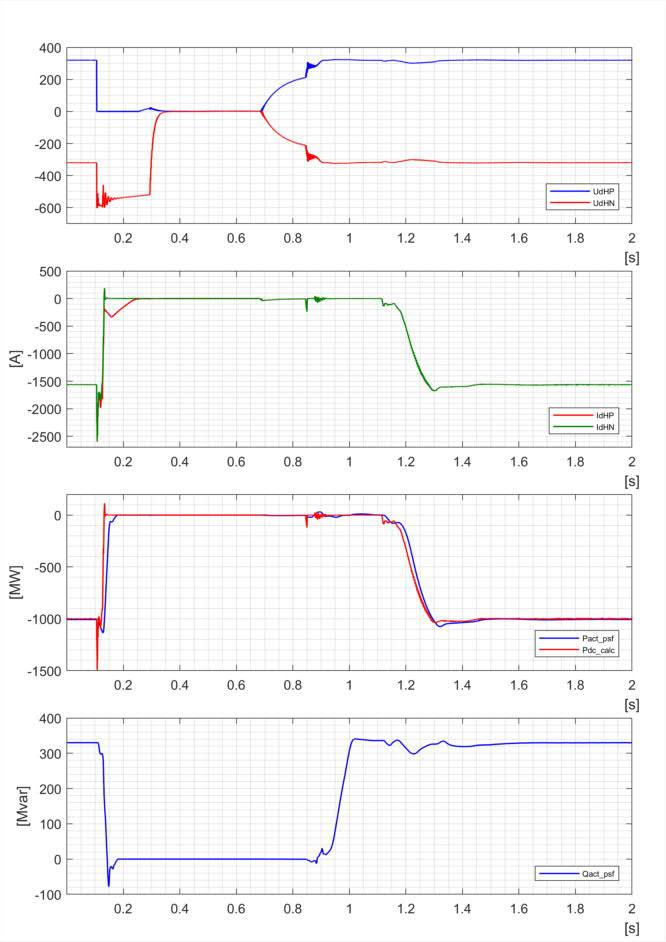
\includegraphics[width=0.6\linewidth]{dc-fault-ride-through/fig/k2026_fig10_simulation_1000mw.png}
  \caption{Dynamic performance study of a pole-to-ground fault on the
           positive pole at 1000\,MW, $+330$\,Mvar; from top: pole voltages,
           pole currents, active power and reactive power. Reproduced
           from~[25], Figure~10}
  \label{fig:dcf-simulation}
\end{figure}

\subsubsection{Pole-to-pole fault record}
\label{sec:dcf-pugalur-pp}

The commissioning record of a pole-to-pole fault in~[24],
Figure~\ref{fig:dcf-pp-record}, shows the fault current fed through the
diode rectifiers after blocking, with the corresponding reactive power drawn
from the AC network as for a three-phase fault with residual voltage. Both
pole voltages collapse to zero without overvoltage and the pole currents
peak at about $-10$\,kA before the breakers open. After the circuit breakers
open the current decays and reaches zero in both stations at
$t_0 + 145$\,ms. The circuit breakers reclose at $t_0 + 850$\,ms and passive
charging begins; station~A deblocks at $t_0 + 1.03$\,s and station~B at
$t_0 + 1.25$\,s, with the same restart procedure as after a pole-to-ground
fault.

\begin{figure}[!ht]
  \centering
  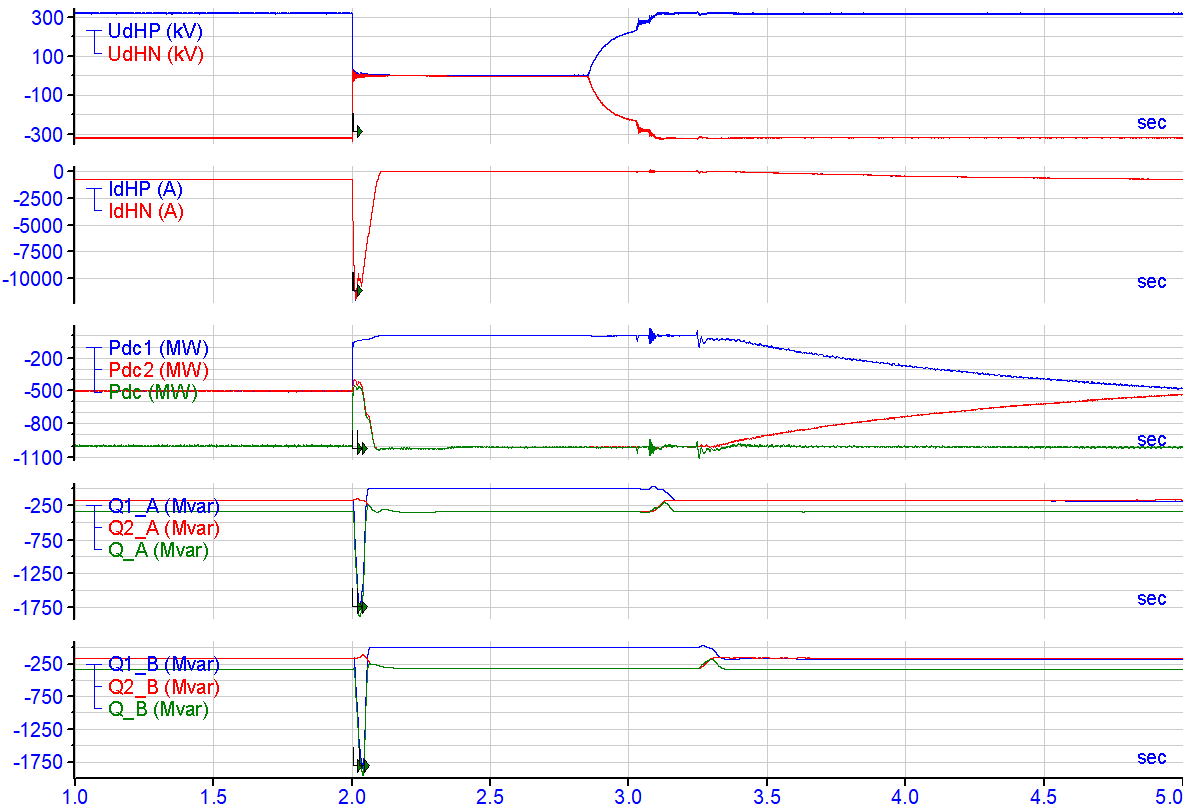
\includegraphics[width=\linewidth]{dc-fault-ride-through/fig/w2022_fig4_pp_recovery.png}
  \caption{Commissioning record of the first restart after a pole-to-pole
           fault on link~1; from top: pole voltages, pole currents, active
           power of link~1, link~2 and total, reactive power at station~A and
           at station~B. Reproduced from~[24], Figure~4}
  \label{fig:dcf-pp-record}
\end{figure}

\subsubsection{Second restart at reduced direct voltage}
\label{sec:dcf-pugalur-reduced}

The commissioning record of a second restart from $\pm$320\,kV to
$\pm$256\,kV, with the other link out of service, shows the power restored
about 60\,s after the fault~[24], Figure~\ref{fig:dcf-reduced-record}; the
time axis of that record spans 70\,s, against 4\,s for the first restarts of
Figures~\ref{fig:dcf-pg-record} and~\ref{fig:dcf-pp-record}. The interval
is the tap-changer movement of Section~\ref{sec:dcf-sequence-reduced}.

\begin{figure}[!ht]
  \centering
  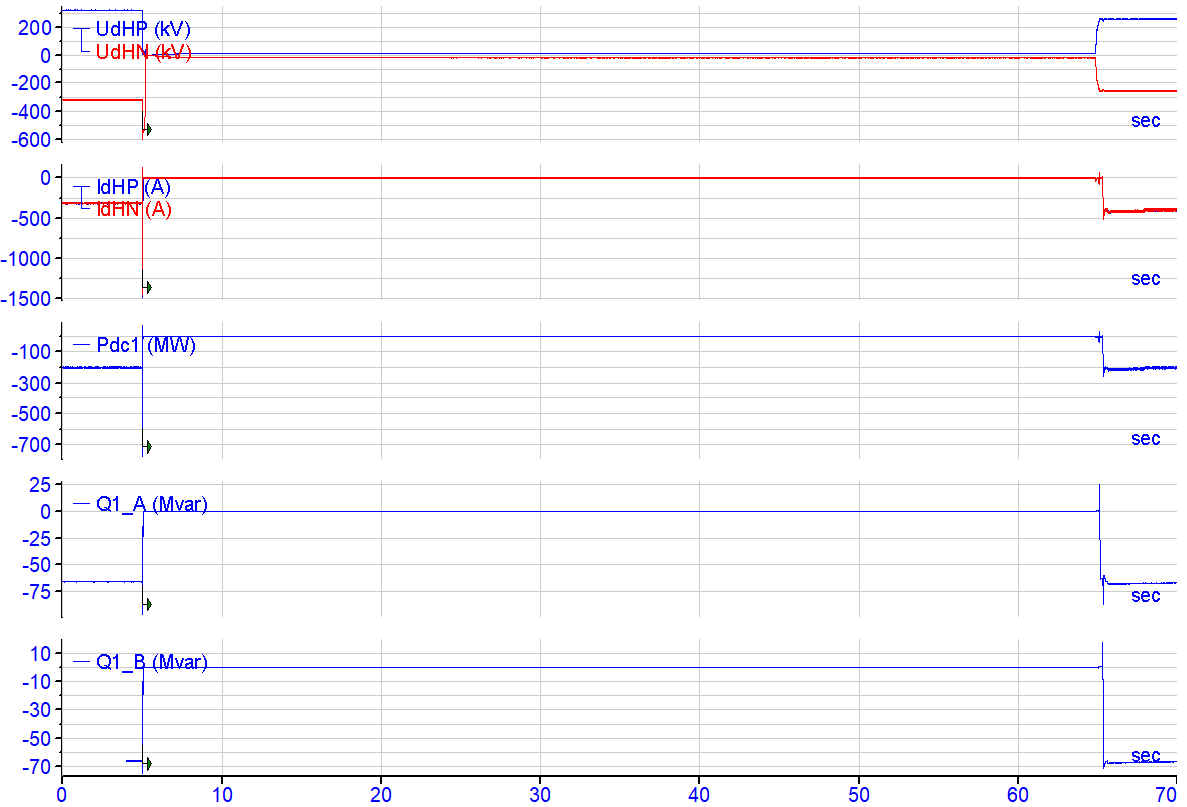
\includegraphics[width=\linewidth]{dc-fault-ride-through/fig/w2022_fig5_reduced_voltage.png}
  \caption{Commissioning record of a second restart to the reduced direct
           voltage of $\pm$256\,kV after a pole-to-ground fault, other link
           out of service; from top: pole voltages, pole currents, active
           power of link~1, reactive power at station~A and at station~B.
           Reproduced from~[24], Figure~5}
  \label{fig:dcf-reduced-record}
\end{figure}

\subsubsection{Permanent fault and changeover to STATCOM operation}
\label{sec:dcf-pugalur-statcom}

Figure~\ref{fig:dcf-permanent} is the commissioning record of a restart
attempt on a permanent pole-to-ground fault, the case of
Section~\ref{sec:dcf-sequence-steps}: after the circuit breaker of
station~A closes, the voltage builds up in the negative pole only, the
currents stay limited by the insertion resistor, the attempt is aborted and
the discharge switch of station~B removes the healthy-pole voltage~[24].

\begin{figure}[!ht]
  \centering
  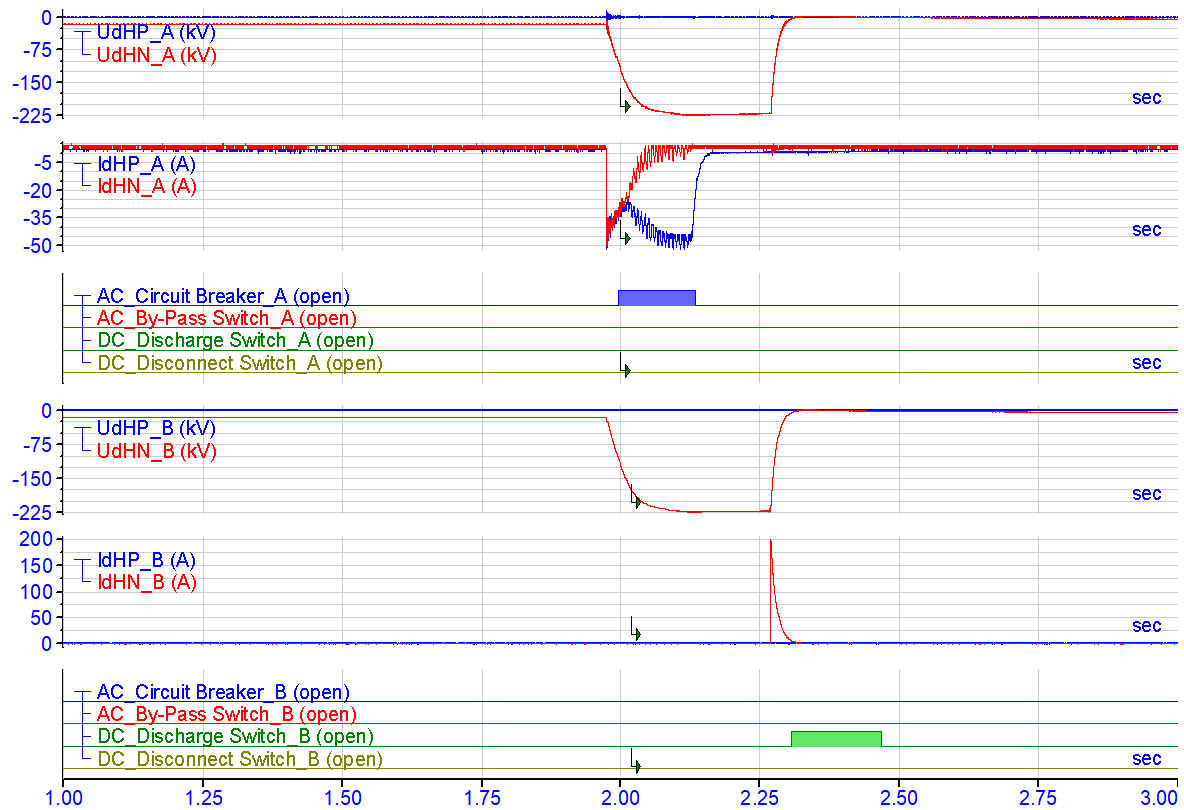
\includegraphics[width=0.9\linewidth]{dc-fault-ride-through/fig/w2022_fig8_permanent_fault.png}
  \caption{Commissioning record of a restart attempt on a permanent
           pole-to-ground fault on the positive pole; for each station the
           pole voltages, pole currents and the positions of circuit breaker,
           bypass switch, discharge switch and DC disconnect switch.
           Reproduced from~[24], Figure~8}
  \label{fig:dcf-permanent}
\end{figure}

Figure~\ref{fig:dcf-statcom-record} is the changeover to STATCOM operation
after a third consecutive pole-to-ground fault. The link was already at
reduced voltage, so the disconnect switches were the only term of the
changeover time of Section~\ref{sec:dcf-zones-statcom}, and both stations
restored reactive power within about 14\,s~[24].

\begin{figure}[!ht]
  \centering
  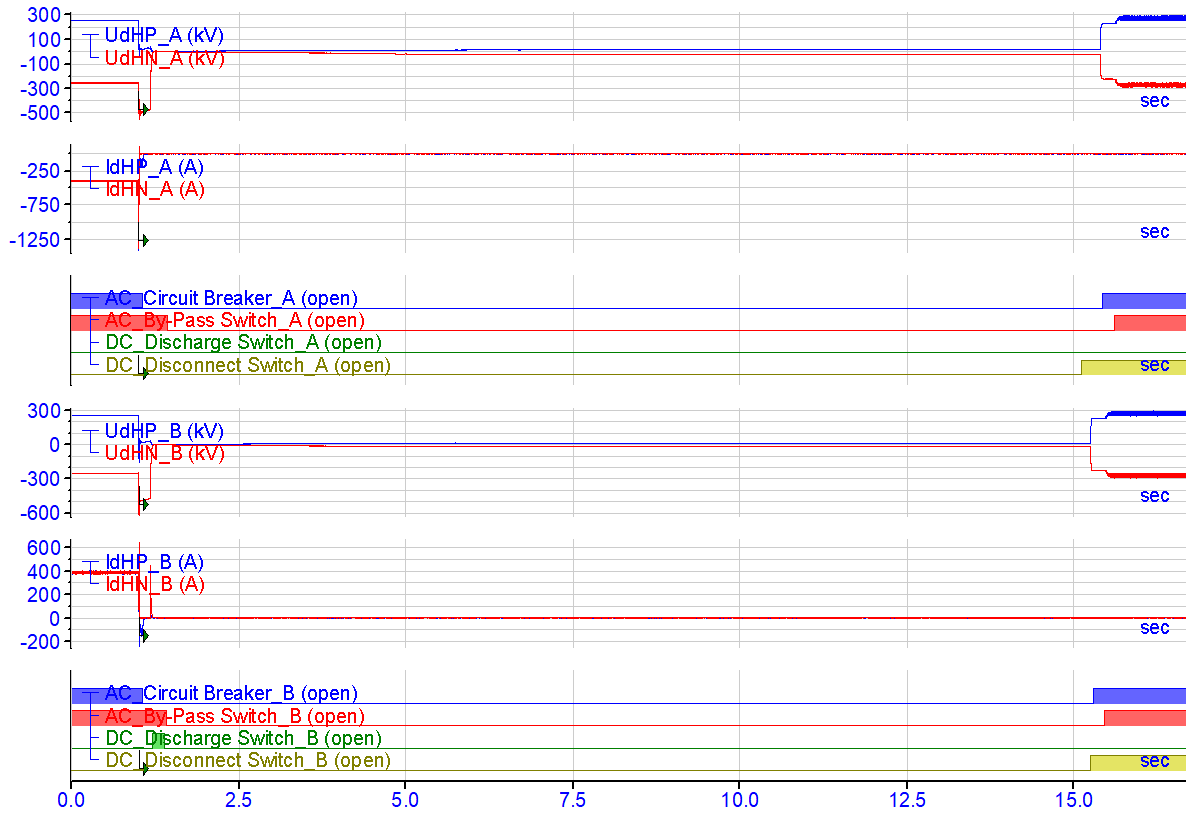
\includegraphics[width=0.9\linewidth]{dc-fault-ride-through/fig/w2022_fig9_statcom_changeover.png}
  \caption{Commissioning record of the changeover to STATCOM operation after
           a third consecutive pole-to-ground fault, link previously at
           reduced direct voltage: the DC disconnect switches open and both
           stations deblock at about 15\,s; for each station the pole
           voltages, pole currents and the switch positions. Reproduced
           from~[24], Figure~9}
  \label{fig:dcf-statcom-record}
\end{figure}

\subsubsection{Cable voltage stresses}
\label{sec:dcf-pugalur-cable}

The commissioning tests were run at short-circuit levels above 10\,GVA and
at a pre-fault power the healthy link could compensate in full~[24].
Measurements at the Thrissur cable termination for faults on the overhead
line near Pugalur, Figure~\ref{fig:dcf-cable-stress}, show the
$\mathrm{d}u/\mathrm{d}t$ of the initial voltage collapse reduced by the
cable impedance, a well damped response to the pole-to-ground fault, and a
first voltage reversal of about 40\,\% for the pole-to-pole fault~[24].

\begin{figure}[!ht]
  \centering
  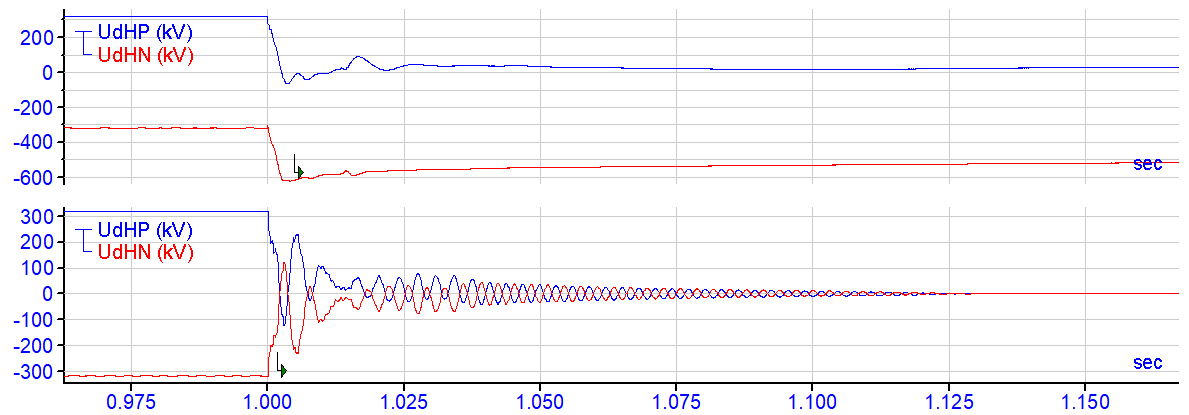
\includegraphics[width=0.9\linewidth]{dc-fault-ride-through/fig/w2022_fig6_cable_stress.png}
  \caption{Pole voltages at the Thrissur cable termination within the first
           150\,ms of a fault on the overhead line near Pugalur: single
           pole-to-ground fault (upper) and pole-to-pole fault (lower).
           Reproduced from~[24], Figure~6}
  \label{fig:dcf-cable-stress}
\end{figure}

\subsubsection{Design decisions of the offer stage}
\label{sec:dcf-pugalur-decisions}

All four alternatives of Section~\ref{sec:dcf-alternatives} were evaluated
at the offer stage of this project and rejected on cost~[24]. Full-bridge
sub-modules and the DC circuit breaker were set aside for their investment
and, for the full bridge, operating losses, and because the lack of
alternative bidders prevented a competitive bidding process. The fixed
no-load voltage was weighed against its 20\,\% higher operating losses, and
the decision was made in favour of the losses, that is for the tap-changer
and the slow second restart. Fast disconnect switches were set aside because
a changeover from rated voltage would not benefit from them, so the
probability of a fast changeover was judged low against their 5- to 10-fold
price. The supplier's assessment after commissioning is that the achieved
recovery times are slightly better than specified, and that the temporary
loss of power is compensated by the parallel link --- a path a single-link
project does not have, Section~\ref{sec:dcf-sequence-compensation}~[24].

\FloatBarrier
